\section{Continuous Random Variables}

\begin{definition}[Cumulative Distribution Function (CDF)]
    For the random variable $X$, is \textit{cumulative distribution function}
    (CDF) $F(X)$ is the function

    \begin{equation}
        \Forall x \in \Real \colon F(X) = \Prob{X \le x}
    \end{equation}

    The CDF has some important properties:
    
    \begin{enumerate}
        \item The CDF $F(X)$ is a \textit{monotonically increasing} function:
        \begin{equation}
            \Forall x, y \in \Real \colon x < y \to F(x) \le F(y)
        \end{equation}
        \item $F(-\infty) = 0$
        \item $F(\infty) = 1$
    \end{enumerate}
    
    If the random variable $X$ is continuous, then its cumulative distribution function $F(X)$ is a continuous function.
\end{definition}

\begin{align}
    \Prob{a < X \le b}
    &= \Prob{X \le b} - \Prob{X \le a} \\
    &= F(b) - F(a)
\end{align}

\begin{definition}[Probability Density Function (PDF)]
    A continuous random variable $X$ has a \textit{probability density function} (PDF) $f(x)$, which is the derivative of the cumulative distribution function $F(x)$
    
    \begin{equation}
        f(x) = \frac{ \dd F(x) }{ \dd x } = F'(x)
    \end{equation}
    
    The probability density function (PDF) $f(x)$ has some important properties:

    \begin{enumerate}
        \item Non-negative range:
        \begin{equation}
            \Forall x \in \Real \colon f(x) \ge 0
        \end{equation}
        \item Inverse of CDF:
        \begin{align}
            \int \limits_{a}^{b} f(x) \dd x
            &= \left[ F(x) \right]_{a}^{b} \\
            &= F(b) - F(a) \\
            &= \Prob{a < X \le b}
        \end{align}
        \item Integrates to $1$:
        \begin{align}
            \int \limits_{-\infty}^{\infty} f(x) \dd x
            &= \Prob{-\infty < X \le +\infty} \\
            &= 1
        \end{align}
    \end{enumerate}
\end{definition}

\begin{remark}
    Note that $f(a) \ne \Prob{X = a}$ because for the continuous random variable $X$, the particular slice at $x = a$ does \textit{not} have a \enquote{thickness} because $\dd x \to 0$.
    
    It is additionally a property that for the continuous random variable $X$
    
    \begin{equation}
        \Forall x \in \Real \colon \Prob{X = x} = 0
    \end{equation}
\end{remark}

\begin{remark}
    The graph of the probability density function can give useful information. The range $[a, b] \in \Real^2$ for which there is a peak in indicates the range of the \textit{mode}, i.e. the most likely value range that $X$ is going to lie in.
\end{remark}

\begin{definition}[Likelihood for Outcome to be within Range]
    For the continuous random variable $X$ over $\Real$, the likelihood that the outcome of a random independent trial takes a value between $[a, b] \in \Real$ where $a \le b$ is given as the definite integral
    
    \begin{align}
        \Prob{a \le X \le b}
        &= \Prob{a < X \le b} \\
        &= \Prob{a \le X < b} \\
        &= \Prob{a < X < b} \\
        &= \int \limits_{a}^{b} f(x) \dd x
    \end{align}
\end{definition}

\subsection{Statistical Measures for Continuous Random Variables}

\begin{definition}[Population Mean]
    For the continuous random variable $X$, its \textit{population mean} $\mu$ is given as
    
    \begin{equation}
        \mu
        = \ExpVal{X}
        = \int \limits_{-\infty}^{\infty} x f(x) \dd x
    \end{equation}
\end{definition}

\begin{definition}[Population Variance]
    For the continuous random variable $X$, its \textit{population variance} $\sigma^2$ is given as
    
    \begin{align}
        \sigma^2
        &= \Var{X} \\
        &= \ExpValS{(X - \mu)^2} \\
        &= \int \limits_{-\infty}^{\infty} (x - \mu)^2 f(x) \dd x \\
        &= \ExpVal{X^2} - \mu^2 \\
        &= \int \limits_{-\infty}^{\infty} x^2 f(x) \dd x - \mu^2
    \end{align}
\end{definition}

\begin{definition}[Expected Value]
    For the continuous random variable $X$ and a function $g(X)$ with $g \colon \Real \to \Real$ from $X$, its \textit{expected value} $\ExpValS{g(X)}$ is given as
    
    \begin{equation}
        \ExpValS{g(X)}
        = \int \limits_{-\infty}^{\infty} g(x) f(x) \dd x
    \end{equation}
\end{definition}

\subsection{Independence}

\begin{definition}[Independence between Two Continuous Random Variables]
    The continuous random variables $X$ and $Y$ are \textit{independent} if and only if
    
    \begin{equation}
        \Forall x, y \in \Real \colon \Prob{X \le x, Y \le y} = \Prob{X \le x} \Prob{Y \le y}
    \end{equation}
\end{definition}

\subsection{Identities over Linear Transformations of the Continuous Random Variable}

\begin{align}
    \ExpVal{a X + b} &= a \ExpVal{X} + b \\
    \Var{a X + b} &= a^2 \Var{X} \\
    \ExpVal{X + Y} &= \ExpVal{X} + \ExpVal{Y} \\
    \ExpVal{X - Y} &= \ExpVal{X} - \ExpVal{Y}
\end{align}

If $X$ and $Y$ are \textit{independent} continuous random variables, then

\begin{equation}
    \Var{X + Y} = \Var{X - Y} = \Var{X} + \Var{Y}
\end{equation}

\subsection{Continuous Distributions}

\subsubsection{Uniform Distribution}

\begin{definition}[Uniform Distribution]
    The \textit{uniform distribution} for the continuous random variable $X$ over the interval $(a, b)$ is denoted $X \sim \Uniform{a}{b}$ where all outcomes in the range are equally likely.

    \begin{figure}[H]
        \centering
        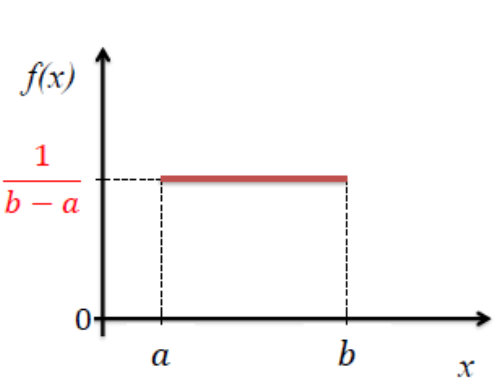
\includegraphics[width=0.3\textwidth]{content/img/4-uniform-pdf.png}
        \caption{Probability Density Function of the Uniform Distribution of Continuous Random Variable $X$ Over the Range $(a, b)$.}
        \label{fig:uniform_pdf}
    \end{figure}
    
    The \textit{probability density function} $f(x)$ for $X \sim \Uniform{a}{b}$ is given by

    \begin{equation}
        f(x) = \begin{cases}
            \frac{1}{b - a} & \text{if $a < x < b$} \\
            0 & \text{otherwise} \\
        \end{cases}
    \end{equation}
    
    The \textit{cumulative density function} $F(x)$ for $X \sim \Uniform{a}{b}$ is given by
    
    \begin{equation}
        F(x) = \Prob{X \le x} = \begin{cases}
            0 & \text{if $x < a$} \\
            \frac{x - a}{b - a} & \text{if $a \le x \le b$} \\
            1 & \text{if $x > b$} \\
        \end{cases}
    \end{equation}
    
    The \textit{mean} of $X \sim \Uniform{a}{b}$ is given by
    
    \begin{equation}
        \ExpVal{X} = \frac{a + b}{2}
    \end{equation}
    
    The \textit{variance} of $X \sim \Uniform{a}{b}$ is given by
    
    \begin{equation}
        \Var{X} = \frac{(b - a)^2}{12}
    \end{equation}
\end{definition}
